\documentclass[uplatex,dvipdfmx,a4paper,twocolumn,base=11pt,jbase=11pt,ja=standard]{bxjsarticle}  % 環境に合わせて変更してください

\usepackage{ipsj}
\usepackage{color}
\usepackage{enumerate}
\usepackage{url}
\usepackage[dvipdfmx]{graphicx}
\usepackage{caption}

\newcommand{\todo}[1]{\colorbox{yellow}{{\bf TODO}:}{\color{red} {\textbf{[#1]}}}}

\title{直観的なScratch作品のためのユーザ入力タイミング特定の試み}{Toward identifying user input timing for intuitive Scratch work search}
\author{和歌山大学}{岡本 圭悟}{Keigo Okamoto, Wakayama University}
\author{和歌山大学}{伊原 彰紀}{Akinori Ihara, Wakayama University}
\author{和歌山大学}{三倉 舞子}{Maiko Mikura, Wakayama University}
\author{和歌山大学}{橋谷 直樹}{Naoki Hashitani, Wakayama University}

\begin{document}
\maketitle

%================
%1
\section{はじめに}
%================

ビジュアルプログラミング言語の学習環境の一つであるScratch\footnote{\url{Scratch: https://scratch.mit.edu/}}では,多様な実装方法を学習/参照するために膨大な作品が公開されており,キーワード検索によって絞り込む機能を有する.
しかし,ユーザが実装したい動作イメージを言語化することは容易でないため,そのイメージに類似する作品の検索は困難である.
従来研究\cite{thesis_fukuchi2021}では,ユーザがイメージするオブジェクトの移動軌跡をマウス操作によって入力し,それをクエリとしてイメージに類似する作品検索を実現しているが,検索にはあらかじめ作品を自動実行してスナップショットを撮影する必要があるため,入力操作を持つ作品は対象にできていない.

本研究の事前分析ではScratchの入力操作を持つ作品数,および実装に必要な計算論理的思考能力をDr.Scratch~\cite{RED2015_J. Moreno-Le ́on}を用いて定量的に計測した.Scratchの入力操作を持つ作品は,入力操作を持たない作品の10倍以上存在する.また,図1は入力操作を持つ作品と入力操作を持たない作品の実装に必要な計算論理的思考のスコア[0-21]の分布を示す.マンホイットニーのU検定より,データ間に有意差があることも示された.このことから,入力操作を持つ作品はより多様な命令処理を必要とすることは明らかである.したがって,入力操作を有する作品を検索の対象に含むべきであるが,入力のタイミングをオブジェクトの移動軌跡のみから判断することは容易でない.

本論文では,入力を有する作品検索に向けて,作品中でユーザが入力操作するタイミングを特定し,自動実行するシステムを提案する.
具体的には,Scratchプログラムから,入力前後の命令処理,入力内容,入力前後のオブジェクトの位置を収集し,ユーザが入力操作するタイミングを特定する.

\begin{figure}
    \begin{center}
        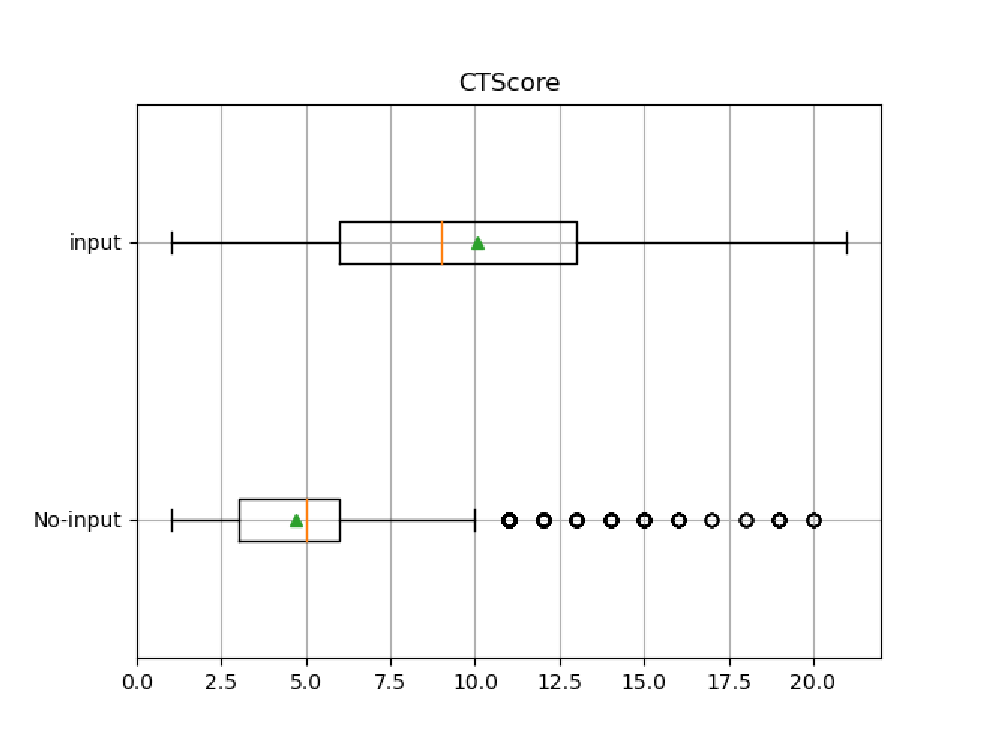
\includegraphics[width=0.9\linewidth]{plot.eps}
        \caption{入力操作をもつ作品と持たない作品のCTスコアの分布}
        \label{fig:test}
    \end{center}
\vspace{-10mm}
\end{figure}

%================
%2
\section{実験}
%================

%2.1
\subsection{データセット}
%================

本論文では,Scratch上で公開されている作品から,以下に示す条件を満たす作品を用いる.
\begin{itemize}
 \item ユーザの操作を有するブロックのうち,文字の入力でないキー入力のみを有するブロックを含む作品
 \item ユーザの定義した変数や関数を含まない作品
 \item 座標移動を行うブロックを含む作品
\end{itemize}

%================
%2.2
\subsection{提案手法}
%================

\noindent\textbf{1. ブロック情報の取得: }対象のScratch作品に含まれる座標ブロック,ユーザの操作を有するブロック,ブロックの実行順序の情報を予め取得しておく.\\
\noindent\textbf{2. 座標の計算: }取得した情報を用いて,作品が実行されてからユーザの操作を有するブロックが処理されるまでにオブジェクトが到達する座標をプログラム上で計算する.\\
\noindent\textbf{3. 入力タイミングの決定: }作品実行時に2.で得た座標に画像オブジェクトが到達したときを入力すべきタイミングとして,自動でキーを押下する.これをスクリプトが処理を終了するまで繰り返す.

「ループブロック」などの制御ブロックはその中の処理が終了したことをスクリプトの処理の終了として扱う.また,並列にスクリプトが存在する場合も同様の手順でスナップショットを撮影する.

%================
%2.4
\subsection{ケーススタディ}
%================

\noindent\textbf{[概要]}本手法で撮影したスナップショットと従来研究で撮影したスナップショットを比べ,どのような動作やブロックを持つ作品が検索の対象になり得るのかを調査する.

\noindent\textbf{[結果]}\todo{結果:従来研究のスナップショットと本手法で撮影したスナップショットを比べて実際にどのような作品が撮影できるようになったのかを記述します}

%
%\subsection{動作実験}
%================

%提案手法を用いてデータセット に含まれる作品20件を実行したところ,全ての作品において入力のタイミングを特定して自動で入力操作を行うことが確認できた.

%================
%3
\section{おわりに}
%================

本論文では,入力を有する作品を含んだ学習者の動作イメージと類似する作品検索に向けて.自動で入力操作を行うタイミングの特定を試みた.今後の方針として,本手法を用いて撮影したスナップショットを用いて実際にどれだけ検索候補の数が向上したかどうかを確かめる.

%================
\section*{謝辞}
%================

\todo{謝辞}

\begin{thebibliography}{1}
  \bibitem{thesis_fukuchi2021} 福地ユキ,伊原彰紀,山本豪志朗,橋谷直樹,オブジェクトの動作に基づくScratch作品の直感的検索手法,\todo{会議名}, 2021
  \bibitem{RED2015_J. Moreno-Le ́on} J. Moreno-Le'on, G. Robles, and M. Rom'an-Gonz'alez, ``Dr. scratch: Automatic analysis of scratch projects to assess and foster computational thinking,'' RED.Revista de Educaci'on a Distancia, vol.15, no.46, pp.1-23, 2015.
  \bibitem{ICMSR2017_Aivaloglou} E. Aivaloglou, F. Hermans, J. Moreno-Le'on, Gr. Robles, ``A dataset of scratch programs: scraped, shaped and scored,'' Proceeding of the International Conference on Mining Software Repositories (MSR'17), pp.511-514, 2017. 

\end{thebibliography}




\bibliographystyle{ipsjunsrt}
%\bibliography{bibfile}

\end{document}
